\documentclass[a4paper]{article}

\bibliographystyle{elsarticle-num}
\usepackage{longtable, caption, listings, xcolor, fancyvrb}
\usepackage{subcaption}
\usepackage{fixltx2e}
\usepackage{amssymb}
\usepackage{amsmath}
\usepackage[margin=1.5in, foot=.25in]{geometry}
\usepackage[labelformat=parens,labelsep=quad,skip=4pt]{caption}
\usepackage{graphicx}
\usepackage[makeroom]{cancel}
\usepackage{enumitem}
\usepackage{float}
\usepackage[colorlinks]{hyperref}
\setlength{\belowcaptionskip}{\baselineskip}

\fvset{frame=single, framesep=2mm,fontfamily=courier,fontsize=\scriptsize, numbers=left,framerule=.3mm,numbersep=2mm,commandchars=\\\{\}}


% \lstset{frame=, basicstyle={\footnotesize\ttfamily}, breaklines=true, postbreak=\mbox{\textcolor{red}{$\hookrightarrow$}\space}, }

\graphicspath{ {images/} }

%-----------------------------------------BEGIN DOC----------------------------------------

\begin{document}

\title{
KRR Project - Documentation {\large\linebreak\\}}
\author{
Dmytro Narepekha\\[0.1cm]
Jianhao Luo\\[0.1cm]
Suzzane Abiri\\[0.1cm]
Sabrila Trifebi Shina\\[0.1cm]
Warsaw University of Technology\\
Faculty of Computer Science and Information Systems\\
}
\date{\today}
\maketitle

\begin{abstract}
The aim of the task was to define an action description language $\mathcal{ADL_{AGP}}$ and corresponding query language $\mathcal{QL_{AGP}}$ that will allow describing a specific group of dynamic systems that takes into account agent-action-program related aspects. 
  Accordingly, this contribution consists of two parts - the theoretical description of the task and the documentation of its practical implementation. 
  In the first part, the introduction provides a brief overview of the task, including the assumptions applied to the corresponding group of dynamic systems. Then, the action description language is defined by means of its syntax and semantics. 
  Following that, the query language is discussed in terms of proposed queries and their satisfiability conditions. 
  Lastly, the theory is concluded with descriptions of various examples that provide an understanding of how the proposed languages can be applied in practice. 
  The second part focuses on the description of the technical aspects of the implemented solution -- i.e. used technology, implemented interface and the performed tests. 
\end{abstract}

\tableofcontents\label{c}
\newpage

\section{Theoretical description}
\subsection{Introduction}
Let \emph{DS\textsubscript{AGP}} be a class of dynamic systems that are the primary focus of this task. \emph{DS\textsubscript{AGP}} fulfills the following assumptions: 
\begin{enumerate}[label=A{{\arabic*}}., leftmargin=*]
    \item \textbf{Inertia law} -- the observed changes, after performing a given action, are only the ones that are directly or indirectly induced by the aforementioned action 
    \item \textbf{Complete information about all actions and all fluents} -- there are no unknown effects of the actions 
    \item \textbf{Determinism} -- there is only one possible outcome of an action 
    \item \textbf{Only sequential actions are allowed} -- the parallel actions are out of consideration 
    \item \textbf{Characteristics of actions}:
        \begin{itemize}
            \item[] $\vartriangleright$ precondition (a set of literals) reflecting a condition under which the action starts and leads to some effect. If a precondition does not hold, then the action is executed with an empty effect
            \item[] $\vartriangleright$ postcondition (a set of literals) reflecting the effect of the action
            \item[] $\vartriangleright$ agent who performs an action
        \end{itemize}
    \item \textbf{State-Dependent Action Constraints for Agents} -- In some states (specified by a propositional formula) some actions cannot be performed by specific agents. 
    \item \textbf{Partial descriptions} -- Partial descriptions of any state of the system (including the initial one) are allowed.
\end{enumerate}
\subsubsection{Task description}
The task of this project is stated as follows:
\begin{quote}
\itshape
Define an action description language \emph{ADL\textsubscript{AGP}} for representing dynamic systems of the class specified above, and define the corresponding query language \emph{QL\textsubscript{AGP}} which would allow getting answers for the following queries:
\begin{enumerate}[label=Q{{\arabic*}}.]
    \item Does a condition $\gamma$ (set of literals) hold after performing a program $\mathcal{P}$?
    \item Is an agent \textit{ag} active in executing a program $\mathcal{P}$?
\end{enumerate}
\end{quote}
%
\subsection{Action description language}
%
Let $\mathcal{ADL_{AGP}}$ be an action description language defined to represent a class of dynamic systems that satisfy the assumptions outlined in the previous section. The following terminology will be used to specify the syntax of the $\mathcal{ADL_{AGP}}$ language: \\~\\
$\Upsilon = (\mathcal{F}, \mathcal{A}_c, \mathcal{A}_g)$ - signature of the language, where:
\begin{itemize}
    \item[-] $\mathcal{F}$ is a set of fluents
    \item[-] $\mathcal{A}_c$ is a set of actions
    \item[-] $\mathcal{A}_g$ is a set of agents
\end{itemize}
$\bar{f}$ - literal corresponding to the fluent $f \in \mathcal{F}$ or its negation $\neg f$ \\[0.5\baselineskip]
$\mathcal{P} = ((A_1, X_1),\dotsc,(A_n, X_n))$ - program, sequence of actions corresponding their agents.
%
\subsubsection{Syntax} \label{statements}
%
Two types of statements were defined for the $\mathcal{ADL_{AGP}}$ language. The first ones are the \textbf{value statements}. They describe the state (more precisely, fluents) that initially holds in the system or holds in the system after performing a particular sequence of actions. The second types of statement are the \textbf{effect statements}. They describe how the system's state changes after performing a given action, namely, what state will result from performing a given action under specified preconditions.
\\ \\
\textbf{\textit{1. Value statements}}
\\ \\
It is important to stress that the second value statement is, in fact, an abbreviation of the first one (i.e. it is not a separate value statement).
\begin{enumerate}
  \item $\Bar{f_1},\dotsc,\Bar{f_k}$ \textbf{after} $(A_1, X_1),\dotsc,(A_n, X_n)$ (where $f_1,\dotsc,f_k\in\mathcal{F}$, $A_1,\dotsc,A_n \in \mathcal{A}_c$, $X_1,\dotsc,X_n \in \mathcal{A}_g$) \\[0.5\baselineskip]
    Meaning: $\Bar{f_1},\dotsc,\Bar{f_k}$ holds after performing a set of actions $(A_1, X_1),\dotsc,(A_n, X_n)$ in the initial state
    \item \textbf{initially} $\Bar{f_1},\dotsc,\Bar{f_k}$ \\[0.5\baselineskip]
    Meaning: $\Bar{f_1},\dotsc,\Bar{f_k}$ holds in the initial state
\end{enumerate}
\textbf{\textit{2. Effect statements}}
\\ \\
Similarly to the previous section, the second effect statement is an abbreviation of the first one. 
The second emphasizes that the action is executed with no specific preconditions that have to be met before its execution.
\begin{enumerate}
  \item A \textbf{causes} $\Bar{f_1},\dotsc,\Bar{f_k}$ by agent \textbf{X} if $\Bar{g_1},\dotsc,\Bar{g_k}$ where $f_1,\dotsc,f_k\in\mathcal{F}$, $g_1,\dotsc,g_k\in\mathcal{F}$ $A\in\mathcal{A}_c$ $a\in\mathcal{A}_g$\\[0.5\baselineskip]
    Meaning: If A is performed in any state satisfying $\Bar{f_1},\dotsc,\Bar{f_k}$ by agent a, then in the resulting state $\Bar{f_1},\dotsc,\Bar{f_k}$ holds. 
    \item A by agent \textbf{X} \textbf{causes} $\Bar{f_1},\dotsc,\Bar{f_k}$ where $f_1,\dotsc,f_k\in\mathcal{F}$\\[0.5\baselineskip]
    Meaning: The performance of action A by agent a leads to the state for which $\alpha$ holds 
\end{enumerate}
%
\subsubsection{Semantics}
%
\textbf{\textit{1. Transition function}}
\\ \\
A \textbf{transition function} is defined as a mapping $\Psi\colon\mathcal{A}_c\times\mathcal{A}_g\times\Sigma\rightarrow\Sigma$. \\
$\Psi(A,X,\sigma)$ defined for any $A\in\mathcal{A}_c$, for any $\sigma\in\Sigma$ and for any $X\in\mathcal{A}_g$ gives a resulting state after performing the action $A$ from the state $\sigma$ by agent X. \\[0.5\baselineskip]
The aforementioned function can also be generalized to the mapping $\Psi^\ast\colon(\mathcal{A}_c \times \mathcal{A}_g)^\ast\times\Sigma\rightarrow\Sigma$ in a following way:
\begin{enumerate}
    \item $\Psi^\ast(\epsilon,\sigma)=\sigma$
    \item $\Psi^\ast(((A_1,X_1),\dotsc,(A_n,X_n)),\sigma)=\Psi((A_n,X_n),\Psi^\ast(((A_1,X_1),\dotsc,(A_{n-1},X_{n-1})),\sigma))$
\end{enumerate}
However, for the sake of simplification, the $\Psi^\ast$ will be further denoted as $\Psi$.
The \textbf{structure} of a language $\mathcal{ADL_{CST}}$ is a pair $S=(\Psi,\sigma_0)$ where $\Psi$ is a transition function and $\sigma_0\in\Sigma$ is the initial state. \\[0.5\baselineskip]
A \textbf{state} is defined as a mapping $\sigma\colon\mathcal{F}\rightarrow\{0, 1\}$, for any $f\in\mathcal{F}$. \\
If $\sigma(f)=1$, then it means that $f$ holds in the state $\sigma$ and it is denoted by $\sigma\models f$. \\
If $\sigma(f)=0$, then it means that $f$ doesn't hold in the state $\sigma$ and it is denoted $\sigma\models\neg f$. \\
Furthermore, let $\Sigma$ denote a set of all states. 
\\ \\
\textbf{\textit{2. Satisfiability of language statements}}
\\ \\
Let $S=(\Psi, \sigma_0)$ be a structure for a language $\mathcal{ADL_{AGP}}$. A statement $s$ is true in $S$ (denoted by $S\models s$), if and only if:
\begin{enumerate}
    \item $s$ is of the form: $\Bar{f_1},\dotsc,\Bar{f_k}$ \textbf{after} $(A_1, X_1),\dotsc,(A_n, X_n)$ \\[0.5\baselineskip]
      $S\models s$ if and only if for an initial state $\sigma_0\in\Sigma$ and the set of actions $A_1,\dotsc,A_n\in\mathcal{A}_c$, the set of agents $X_1,\dotsc,X_n\in\mathcal{A}_g$ the following holds: 
    $\Psi^\ast(((A_1,X_1),\dotsc,(A_n,X_n)),\sigma_0)\models\Bar{f_1},\dotsc,\Bar{f_k}$
    \item $s$ is of the form: A \textbf{causes} $\Bar{f_1},\dotsc,\Bar{f_k}$  by agent X if $\Bar{g_1},\dotsc,\Bar{g_k}$   \\[0.5\baselineskip]
    $S\models s$ if and only if for every state $\sigma\in\Sigma$ such that $\sigma\models\Bar{g_1},\dotsc,\Bar{g_k}$ and the action $A\in\mathcal{A}_c$, the agent $X\in\mathcal{A}_g$, the following holds: 
    $\Psi^\ast(A, X,\sigma)\models\Bar{f_1},\dotsc,\Bar{f_k}$ 
\end{enumerate}
\textbf{\textit{3. Model of a language}}
\\ \\
Let D be an action domain (non-empty set of value or effect statements) in the language $\mathcal{ADL_{AGP}}$ over a signature $\Upsilon = (\mathcal{F}, \mathcal{A}_c, \mathcal{A}_g)$. 
A structure for this language $S=(\Psi,\sigma_0)$ is a model of D if and only if:
\begin{enumerate}
    \item for every $s \in D$, $S \models s$
    \item for every $A\in\mathcal{A}_c$, for every $\Bar{f_1},\dotsc,\Bar{f_k},g_1,\dotsc,g_k\in\mathcal{F}$, for every $\sigma\in\Sigma$, for every $X\in\mathcal{A_g}$ if one of the following conditions holds:
    \begin{enumerate}[label=(\alph*)]
      \item there is a statement in D of the form A \textbf{causes} $\Bar{f_1},\dotsc,\Bar{f_k}$ by agent X if $\Bar{g_1},\dotsc,\Bar{g_k}$ such that $\sigma \cancel{\models} \Bar{f_i}$ for some $i = 1,\dotsc,k$
        \item D does not contain an effect statement A \textbf{causes} $\Bar{f}$ if $\Bar{g_1},\dotsc,\Bar{g_k}$ 
    \end{enumerate}
    then $\sigma\models \Bar{f_1},\dotsc,\Bar{f_k}$ if and only if $\Psi(A,a,\sigma) \models \Bar{f_1},\dotsc,\Bar{f_k}$
\end{enumerate}
%
\subsection{Query Language}
%
Let $\mathcal{QL_{AGP}}$ be the query language corresponding to the $\mathcal{ADL_{AGP}}$. 
%
\subsubsection{Query statements}
%
There were two types of queries defined for $\mathcal{QL_{CST}}$, namely the \textbf{value queries} and \textbf{active queries}. The value queries answer the question of whether a given condition is satisfied after performing a sequence of actions. The active queries evaluate if a given agent  is active for execution of sequence of actions.
\\[0.5\baselineskip]
\textbf{\textit{1. Value queries}}
\\[0.5\baselineskip]
The value query is defined in the following way:\\[0.5\baselineskip]
 $\Bar{f_1},\dotsc,\Bar{f_k}$ \textbf{after} $(A_1, X_1),\dotsc,(A_n, X_n)$ \\[0.5\baselineskip] 
Meaning: does the condition $\Bar{f_1},\dotsc,\Bar{f_k}$ hold after executing the sequence of actions $(A_1, X_1),\dotsc,(A_n, X_n)$
\\\\
\textbf{\textit{2. Active queries}}
\\[0.5\baselineskip]
\textbf{active} X in $(A_1, X_1),\dotsc,(A_n, X_n)$\\[0.5\baselineskip] 
Meaning: is the agent X active in the program $(A_1, X_1),\dotsc,(A_n, X_n)$?  \\[0.5\baselineskip]

\subsubsection{Satisfiability of queries}
Let $D$ be an action domain. A query $Q$ is a consequence of $D$, denoted by $D \models Q$, if and only if $Q$ is true in every model S=$(\Psi, \sigma_0)$ of $D$:
\begin{enumerate}
  \item Q is of the form: $\Bar{f_1},\dotsc,\Bar{f_k}$ \textbf{after} $(A_1, X_1),\dotsc,(A_n, X_n)$ \\[0.5\baselineskip] 
    $D \models Q$ if and only if for any model $S=(\Psi,\sigma_0)$ of $D$, 
   the following holds $\Psi(((A_1,X_1),\dotsc,(A_n,X_n)),\sigma_0)\models \Bar{f_i}$ for every i = $1, \dotsc, k$
  \item Q is of the form: \textbf{active} X in $(A_1, X_1),\dotsc,(A_n, X_n)$\\[0.5\baselineskip] 
    $D \models Q$ if and only if for any model $S=(\Psi,\sigma_0)$ of $D$ 
    there exists i =1, 2, 3 \ldots, j, such that 
    \begin{enumerate}
      \item X = $X_i$
      \item $\sigma_i \neq \sigma_{i-1}$ and where $\sigma_j$ = $\Psi((A_1, X_1),\dotsc,(A_j, X_j),\sigma_0)$ $j = 1, \dotsc, n$     
    \end{enumerate}
\end{enumerate}
\section{Examples of dynamic systems}
\subsubsection{Online store Scenario}
An online store sells housing materials.The following literals can describe the status of the product: ordered, shipped and delivered.
Initially, the product is neither ordered nor shipped. 
Purchasing the product makes it ordered, shipping the product makes it shipped, and, lastly, delivering the product makes it delivered. 
Each action has an associated agent attached if the initial conditions for performing a specific action are met. \\\\
\begin{tabular}{|l|c|r|}
\hline
\textbf{Fluent} & \textbf{literal} & \textbf{nagation} \\ \hline
$f_1$ & Ordered & $\neg$Ordered \\
$f_2$ & Shipped & $\neg$Shipped \\
$f_3$ & Delivered & $\neg$Delivered \\ \hline
\end{tabular} \\\\
Actions are defined as:
\begin{enumerate}
  \item Purchase
  \item Ship
  \item Deliver
\end{enumerate}
Agents:
\begin{enumerate}
  \item \textbf{Buyer}: Can only perform action: \textbf{Purchase}
  \item \textbf{Seller}: Can only perform action: \textbf{Ship} and \textbf{Deliver}
\end{enumerate}
Agents perform undefined actions will have no effect.
The set of all considered states in this scenario is defined as: \\\\
$\Sigma = \{{\sigma_0, \sigma_1, \sigma_2, \sigma_3, \sigma_4, \sigma_5, \sigma_6, \sigma_7\}}$, where:
\begin{center}
$\sigma_0 = \{${$\neg$ordered, $\neg$shipped, $\neg$delivered}\} \\[0.1\baselineskip]
$\sigma_1 = \{${ordered, $\neg$shipped, $\neg$delivered}\} \\[0.1\baselineskip]
$\sigma_2 = \{${$\neg$ordered, shipped, $\neg$delivered}\} \\[0.1\baselineskip]
$\sigma_3 = \{${ordered, shipped, delivered}\} \\[0.1\baselineskip]
$\sigma_4 = \{${$\neg$ordered, $\neg$shipped, delivered}\} \\[0.1\baselineskip]
$\sigma_5 = \{${$\neg$ordered, shipped, delivered}\} \\[0.1\baselineskip]
$\sigma_6 = \{${ordered, $\neg$shipped, delivered}\} \\[0.1\baselineskip]
$\sigma_7 = \{${$\neg$ordered, shipped, $\neg$delivered}\} \\[0.1\baselineskip]
\end{center}

The structure of the scenario is as follows:
\begin{center}
\textbf{initially} $\neg$\textit{ordered} \\[0.1\baselineskip]
\textbf{initially} $\neg$\textit{shipped} \\[0.1\baselineskip]
\textbf{initially} $\neg$\textit{delivered} \\[0.1\baselineskip]
\textit{Purchase} by \textit{Buyer} \textbf{causes} \textit{ordered} \textbf{if} $\neg$\textit{ordered} $\neg$\textit{shipped} $\neg$\textit{delivered}\\[0.1\baselineskip]
\textit{Ship} by \textit{Seller} \textbf{causes} \textit{shipped} \textbf{if} \textit{ordered}, $\neg$\textit{shipped} $\neg$\textit{delivered}\\[0.1\baselineskip]
\textit{Deliver} by \textit{Seller} \textbf{causes} \textit{delivered} \textbf{if} \textit{shipped}, \textit{ordered}, $\neg$\textit{delivered} \\[0.5\baselineskip]
\end{center}
Hence, the following states are considered in this case: \\[0.5\baselineskip] 
$\Psi((\text{Purchase},\text{Buyer}),\sigma_0)$ = $\sigma_1$ \\[0.1\baselineskip] 
$\Psi((\text{Purchase},\text{Seller}),\sigma_0)$ = $\sigma_0$ \\[0.1\baselineskip] 
$\Psi((\text{Ship},\text{Buyer}),\sigma_0)$ = $\sigma_0$ \\[0.1\baselineskip] 
$\Psi((\text{Ship},\text{Seller}),\sigma_0)$ = $\sigma_0$ \\[0.1\baselineskip] 
$\Psi((\text{Deliver}, \text{Buyer}),\sigma_0)$ = $\sigma_0$ \\[0.1\baselineskip]
$\Psi((\text{Deliver}, \text{Seller}),\sigma_0)$ = $\sigma_0$ \\[0.7\baselineskip]
$\Psi((\text{Purchase},\text{Buyer}),\sigma_1)$ = $\sigma_1$ \\[0.1\baselineskip] 
$\Psi((\text{Purchase},\text{Seller}),\sigma_1)$ = $\sigma_1$ \\[0.1\baselineskip] 
$\Psi((\text{Ship},\text{Buyer}),\sigma_1)$ = $\sigma_1$ \\[0.1\baselineskip] 
$\Psi((\text{Ship},\text{Seller}),\sigma_1)$ = $\sigma_2$ \\[0.1\baselineskip] 
$\Psi((\text{Deliver},\text{Buyer}),\sigma_1)$ = $\sigma_1$ \\[0.1\baselineskip] 
$\Psi((\text{Deliver},\text{Seller}),\sigma_1)$ = $\sigma_1$ \\[0.7\baselineskip] 
$\Psi((\text{Purchase},\text{Buyer}),\sigma_2)$ = $\sigma_2$ \\[0.1\baselineskip] 
$\Psi((\text{Purchase},\text{Seller}),\sigma_2)$ = $\sigma_2$ \\[0.1\baselineskip] 
$\Psi((\text{Ship},\text{Seller}),\sigma_2)$ = $\sigma_2$ \\[0.1\baselineskip] 
$\Psi((\text{Ship},\text{Buyer}),\sigma_2)$ = $\sigma_2$ \\[0.1\baselineskip] 
$\Psi((\text{Deliver},\text{Buyer}),\sigma_2)$ = $\sigma_2$ \\[0.1\baselineskip] 
$\Psi((\text{Deliver},\text{Seller}),\sigma_2)$ = $\sigma_3$ \\[0.7\baselineskip] 
$\Psi((\text{Purchase},\text{Buyer}),\sigma_3)$ = $\sigma_3$ \\[0.1\baselineskip] 
$\Psi((\text{Purchase},\text{Seller}),\sigma_3)$ = $\sigma_3$ \\[0.1\baselineskip] 
$\Psi((\text{Ship},\text{Buyer}),\sigma_3)$ = $\sigma_3$ \\[0.1\baselineskip] 
$\Psi((\text{Ship},\text{Seller}),\sigma_3)$ = $\sigma_3$ \\[0.1\baselineskip] 
$\Psi((\text{Deliver},\text{Buyer}),\sigma_3)$ = $\sigma_3$ \\[0.1\baselineskip] 
$\Psi((\text{Deliver},\text{Seller}),\sigma_3)$ = $\sigma_3$ \\[0.7\baselineskip] 
$\Psi((\text{Purchase},\text{Buyer}),\sigma_4)$ = $\sigma_4$ \\[0.1\baselineskip] 
$\Psi((\text{Purchase},\text{Seller}),\sigma_4)$ = $\sigma_4$ \\[0.1\baselineskip] 
$\Psi((\text{Ship},\text{Buyer}),\sigma_4)$ = $\sigma_4$ \\[0.1\baselineskip] 
$\Psi((\text{Ship},\text{Seller}),\sigma_4)$ = $\sigma_4$ \\[0.1\baselineskip] 
$\Psi((\text{Deliver},\text{Buyer}),\sigma_4)$ = $\sigma_4$ \\[0.1\baselineskip] 
$\Psi((\text{Deliver},\text{Seller}),\sigma_4)$ = $\sigma_4$ \\[0.7\baselineskip] 
$\Psi((\text{Purchase},\text{Buyer}),\sigma_5)$ = $\sigma_5$ \\[0.1\baselineskip] 
$\Psi((\text{Purchase},\text{Seller}),\sigma_5)$ = $\sigma_5$ \\[0.1\baselineskip] 
$\Psi((\text{Ship},\text{Buyer}),\sigma_5)$ = $\sigma_5$ \\[0.1\baselineskip] 
$\Psi((\text{Ship},\text{Seller}),\sigma_5)$ = $\sigma_5$ \\[0.1\baselineskip] 
$\Psi((\text{Deliver},\text{Buyer}),\sigma_5)$ = $\sigma_5$ \\[0.1\baselineskip] 
$\Psi((\text{Deliver},\text{Seller}),\sigma_5)$ = $\sigma_5$ \\[0.7\baselineskip] 
$\Psi((\text{Purchase},\text{Buyer}),\sigma_6)$ = $\sigma_6$ \\[0.1\baselineskip] 
$\Psi((\text{Purchase},\text{Seller}),\sigma_6)$ = $\sigma_6$ \\[0.1\baselineskip] 
$\Psi((\text{Ship},\text{Buyer}),\sigma_6)$ = $\sigma_6$ \\[0.1\baselineskip] 
$\Psi((\text{Ship},\text{Seller}),\sigma_6)$ = $\sigma_6$ \\[0.1\baselineskip] 
$\Psi((\text{Deliver},\text{Buyer}),\sigma_6)$ = $\sigma_6$ \\[0.1\baselineskip] 
$\Psi((\text{Deliver},\text{Seller}),\sigma_6)$ = $\sigma_6$ \\[0.7\baselineskip] 
$\Psi((\text{Purchase},\text{Buyer}),\sigma_7)$ = $\sigma_7$ \\[0.1\baselineskip] 
$\Psi((\text{Purchase},\text{Seller}),\sigma_7)$ = $\sigma_7$ \\[0.1\baselineskip] 
$\Psi((\text{Ship},\text{Buyer}),\sigma_7)$ = $\sigma_7$ \\[0.1\baselineskip] 
$\Psi((\text{Ship},\text{Seller}),\sigma_7)$ = $\sigma_7$ \\[0.1\baselineskip] 
$\Psi((\text{Deliver},\text{Buyer}),\sigma_7)$ = $\sigma_7$ \\[0.1\baselineskip] 
$\Psi((\text{Deliver},\text{Seller}),\sigma_7)$ = $\sigma_7$ \\[0.7\baselineskip] 
Figure~\ref{fig:shipping_transitions} outlines all of the aforementioned transitions.
\begin{figure}[H]
    \centering
    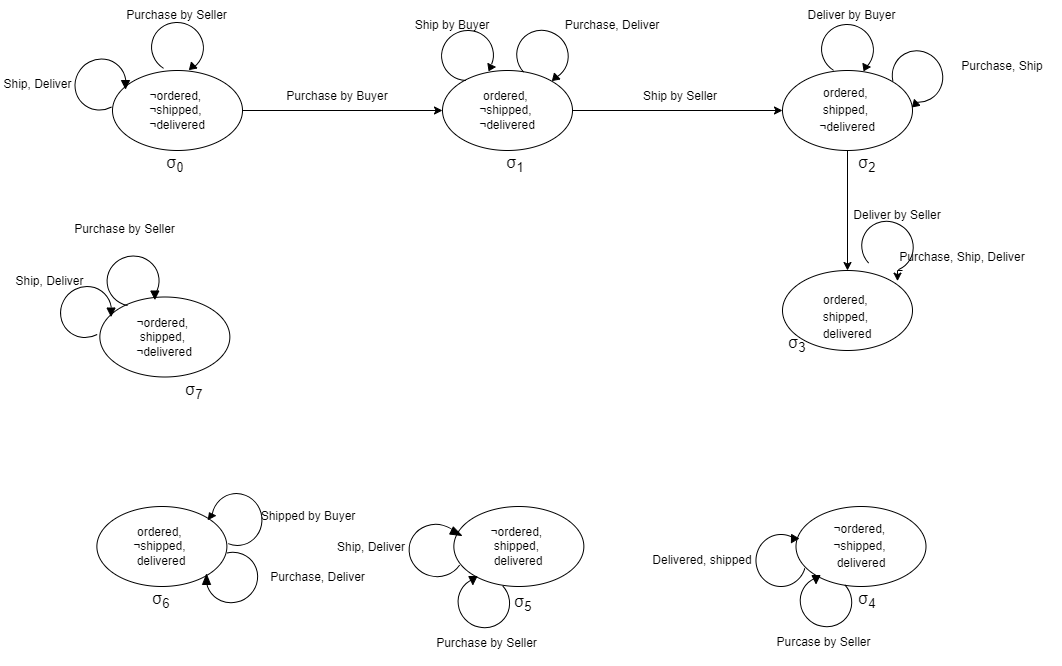
\includegraphics[width=1\linewidth]{onlinestore.png}
    \caption{Shipping orders - all possible transitions}
    \label{fig:shipping_transitions}
\end{figure}
Let us demonstrate an example of asking queries using the structure of the query language $\mathcal{QL_{CST}}$. 
Assume, that the initial state is $\sigma_0$ and the program $\mathcal{P}$ = ((\textit{Purchase}, \textit{Buyer}),(\textit{Ship}, \textit{Seller}), (\textit{Deliver}, \textit{Seller}).
Let us consider the following query statements:
\begin{enumerate}
  \item $\neg$\textit{delivered} \textbf{after} ((\textit{Purchase}, \textit{Buyer}),(\textit{Ship}, \textit{Seller}), (\textit{Deliver}, \textit{Seller})).
  \item \textbf{Active} Seller \textbf{in} ((\textit{Purchase}, \textit{Buyer}),(\textit{Ship}, \textit{Seller}), (\textit{Deliver}, \textit{Seller})).
\end{enumerate}
The program execution will consist of the following transitions: \\[0.5\baselineskip]
$\Psi((\text{Purchase},Buyer),\sigma_0)$ = $\sigma_1$ \\[0.1\baselineskip]
$\Psi((\text{Ship},Seller),\sigma_1)$ = $\sigma_2$ \\[0.1\baselineskip]
$\Psi((\text{Deliver},Seller),\sigma_2)$ = $\sigma_3$ \\[0.7\baselineskip]
As it can be observed, after the program execution, the state $\sigma_3$ will hold. Due to that, query number one will retrieve a negative response (i.e. \textit{false}), 
as in the final state \textit{delivered} holds. 
On the other hand, the second query will respond with \textit{true} as  action performed by Agent \textit{Seller} did changed the state of $\sigma_1$ into $\sigma_2$ and the $\sigma_2$ into $\sigma_3$.
\subsubsection{Coffee Order Scenario}
In this scenario, the status of the order can be describe by the following fluents: received, brewed, and served. 
Initially the order is not received, the coffee is not brewed, and is not served. 
There will be 3 actions that can be executed: receive order, brew and serve. 
Receive order makes it received, brew an order makes it brewed, and serve makes it served the order. 
Each of those aforementioned actions has associated agent attached in case the initial conditions performing a specific action are met.
\\\\
\begin{tabular}{|l|c|r|}
\hline
\textbf{Fluent} & \textbf{literal} & \textbf{nagation} \\ \hline
$f_1$ & Received & $\neg$Received \\
$f_2$ & Brewed & $\neg$Brewed \\
$f_3$ & Served & $\neg$Served \\ \hline
\end{tabular} \\\\
Actions are defined as:
\begin{enumerate}
  \item Receive Order
  \item Brew
  \item Serve
\end{enumerate}
Agents:
\begin{enumerate}
  \item \textbf{Cashier}: Can only perform action: \textbf{Receive Order}
  \item \textbf{Barista}: Can only perform action: \textbf{Brew} and \textbf{Serve}
\end{enumerate}
Agents perform undefined actions will have no effect.
The set of all considered states in this scenario is defined as: \\\\
$\Sigma = \{{\sigma_0, \sigma_1, \sigma_2, \sigma_3, \sigma_4, \sigma_5, \sigma_6, \sigma_7\}}$, where:
\begin{center}
$\sigma_0 = \{${$\neg$received, $\neg$brewed, $\neg$served}\} \\[0.1\baselineskip]
$\sigma_1 = \{${received, $\neg$brewed, $\neg$served}\} \\[0.1\baselineskip]
$\sigma_2 = \{${received, brewed, $\neg$served}\} \\[0.1\baselineskip]
$\sigma_3 = \{${received, brewed, served}\} \\[0.1\baselineskip]
$\sigma_4 = \{${$\neg$received, $\neg$brewed, served}\} \\[0.1\baselineskip]
$\sigma_5 = \{${$\neg$received, brewed, served}\} \\[0.1\baselineskip]
$\sigma_6 = \{${received, $\neg$brewed, served}\} \\[0.1\baselineskip]
$\sigma_7 = \{${$\neg$received, brewed, $\neg$served}\} \\[0.1\baselineskip]
\end{center}

The structure of the scenario is as follows:
\begin{center}
\textbf{initially} $\neg$\textit{received} \\[0.1\baselineskip]
\textbf{initially} $\neg$\textit{brewed} \\[0.1\baselineskip]
\textbf{initially} $\neg$\textit{served} \\[0.1\baselineskip]
\textit{Receive Order} by \textit{Cashier} \textbf{causes} \textit{received} \textbf{if} $\neg$\textit{received} $\neg$\textit{brewed} $\neg$\textit{served}\\[0.1\baselineskip]
\textit{Brew} by \textit{Barista} \textbf{causes} \textit{brewed} \textbf{if} \textit{received}, $\neg$\textit{brewed} $\neg$\textit{served}\\[0.1\baselineskip]
\textit{Serve} by \textit{Barista} \textbf{causes} \textit{served} \textbf{if} \textit{received}, \textit{brewed}, $\neg$\textit{served} \\[0.5\baselineskip]
\end{center}
Hence, the following states are considered in this case: \\[0.5\baselineskip] 
$\Psi((\text{Receive Order},\text{Cashier}),\sigma_0)$ = $\sigma_1$ \\[0.1\baselineskip] 
$\Psi((\text{Receive Order},\text{Barista}),\sigma_0)$ = $\sigma_0$ \\[0.1\baselineskip] 
$\Psi((\text{Brew},\text{Cashier}),\sigma_0)$ = $\sigma_0$ \\[0.1\baselineskip] 
$\Psi((\text{Brew},\text{Barista}),\sigma_0)$ = $\sigma_0$ \\[0.1\baselineskip] 
$\Psi((\text{Serve}, \text{Cashier}),\sigma_0)$ = $\sigma_0$ \\[0.1\baselineskip]
$\Psi((\text{Serve}, \text{Barista}),\sigma_0)$ = $\sigma_0$ \\[0.7\baselineskip]
$\Psi((\text{Receive Order},\text{Cashier}),\sigma_1)$ = $\sigma_1$ \\[0.1\baselineskip] 
$\Psi((\text{Receive Order},\text{Barista}),\sigma_1)$ = $\sigma_1$ \\[0.1\baselineskip] 
$\Psi((\text{Brew},\text{Cashier}),\sigma_1)$ = $\sigma_1$ \\[0.1\baselineskip] 
$\Psi((\text{Brew},\text{Barista}),\sigma_1)$ = $\sigma_2$ \\[0.1\baselineskip] 
$\Psi((\text{Serve},\text{Cashier}),\sigma_1)$ = $\sigma_1$ \\[0.1\baselineskip] 
$\Psi((\text{Serve},\text{Barista}),\sigma_1)$ = $\sigma_1$ \\[0.7\baselineskip] 
$\Psi((\text{Receive Order},\text{Cashier}),\sigma_2)$ = $\sigma_2$ \\[0.1\baselineskip] 
$\Psi((\text{Receive Order},\text{Barista}),\sigma_2)$ = $\sigma_2$ \\[0.1\baselineskip] 
$\Psi((\text{Brew},\text{Cashier}),\sigma_2)$ = $\sigma_2$ \\[0.1\baselineskip] 
$\Psi((\text{Brew},\text{Barista}),\sigma_2)$ = $\sigma_2$ \\[0.1\baselineskip] 
$\Psi((\text{Serve},\text{Cashier}),\sigma_2)$ = $\sigma_2$ \\[0.1\baselineskip] 
$\Psi((\text{Serve},\text{Barista}),\sigma_2)$ = $\sigma_3$ \\[0.7\baselineskip] 
$\Psi((\text{Receive Order},\text{Cashier}),\sigma_3)$ = $\sigma_3$ \\[0.1\baselineskip] 
$\Psi((\text{Receive Order},\text{Barista}),\sigma_3)$ = $\sigma_3$ \\[0.1\baselineskip] 
$\Psi((\text{Brew},\text{Cashier}),\sigma_3)$ = $\sigma_3$ \\[0.1\baselineskip] 
$\Psi((\text{Brew},\text{Barista}),\sigma_3)$ = $\sigma_3$ \\[0.1\baselineskip] 
$\Psi((\text{Serve},\text{Cashier}),\sigma_3)$ = $\sigma_3$ \\[0.1\baselineskip] 
$\Psi((\text{Serve},\text{Barista}),\sigma_3)$ = $\sigma_3$ \\[0.7\baselineskip] 
$\Psi((\text{Receive Order},\text{Cashier}),\sigma_4)$ = $\sigma_4$ \\[0.1\baselineskip] 
$\Psi((\text{Receive Order},\text{Barista}),\sigma_4)$ = $\sigma_4$ \\[0.1\baselineskip] 
$\Psi((\text{Brew},\text{Cashier}),\sigma_4)$ = $\sigma_4$ \\[0.1\baselineskip] 
$\Psi((\text{Brew},\text{Barista}),\sigma_4)$ = $\sigma_4$ \\[0.1\baselineskip] 
$\Psi((\text{Serve},\text{Cashier}),\sigma_4)$ = $\sigma_4$ \\[0.1\baselineskip] 
$\Psi((\text{Serve},\text{Barista}),\sigma_4)$ = $\sigma_4$ \\[0.7\baselineskip] 
$\Psi((\text{Receive Order},\text{Cashier}),\sigma_5)$ = $\sigma_5$ \\[0.1\baselineskip] 
$\Psi((\text{Receive Order},\text{Barista}),\sigma_5)$ = $\sigma_5$ \\[0.1\baselineskip] 
$\Psi((\text{Brew},\text{Cashier}),\sigma_5)$ = $\sigma_5$ \\[0.1\baselineskip] 
$\Psi((\text{Brew},\text{Barista}),\sigma_5)$ = $\sigma_5$ \\[0.1\baselineskip] 
$\Psi((\text{Serve},\text{Cashier}),\sigma_5)$ = $\sigma_5$ \\[0.1\baselineskip] 
$\Psi((\text{Serve},\text{Barista}),\sigma_5)$ = $\sigma_5$ \\[0.7\baselineskip] 
$\Psi((\text{Receive Order},\text{Cashier}),\sigma_6)$ = $\sigma_6$ \\[0.1\baselineskip] 
$\Psi((\text{Receive Order},\text{Barista}),\sigma_6)$ = $\sigma_6$ \\[0.1\baselineskip] 
$\Psi((\text{Brew},\text{Cashier}),\sigma_6)$ = $\sigma_6$ \\[0.1\baselineskip] 
$\Psi((\text{Brew},\text{Barista}),\sigma_6)$ = $\sigma_6$ \\[0.1\baselineskip] 
$\Psi((\text{Serve},\text{Cashier}),\sigma_6)$ = $\sigma_6$ \\[0.1\baselineskip] 
$\Psi((\text{Serve},\text{Barista}),\sigma_6)$ = $\sigma_6$ \\[0.7\baselineskip] 
$\Psi((\text{Receive Order},\text{Cashier}),\sigma_7)$ = $\sigma_7$ \\[0.1\baselineskip] 
$\Psi((\text{Receive Order},\text{Barista}),\sigma_7)$ = $\sigma_7$ \\[0.1\baselineskip] 
$\Psi((\text{Brew},\text{Cashier}),\sigma_7)$ = $\sigma_7$ \\[0.1\baselineskip] 
$\Psi((\text{Brew},\text{Barista}),\sigma_7)$ = $\sigma_7$ \\[0.1\baselineskip] 
$\Psi((\text{Serve},\text{Cashier}),\sigma_7)$ = $\sigma_7$ \\[0.1\baselineskip] 
$\Psi((\text{Serve},\text{Barista}),\sigma_7)$ = $\sigma_7$ \\[0.7\baselineskip] 
Figure~\ref{fig:coffee_order_transactions} outlines all of the aforementioned transitions.
\begin{figure}[H]
    \centering
    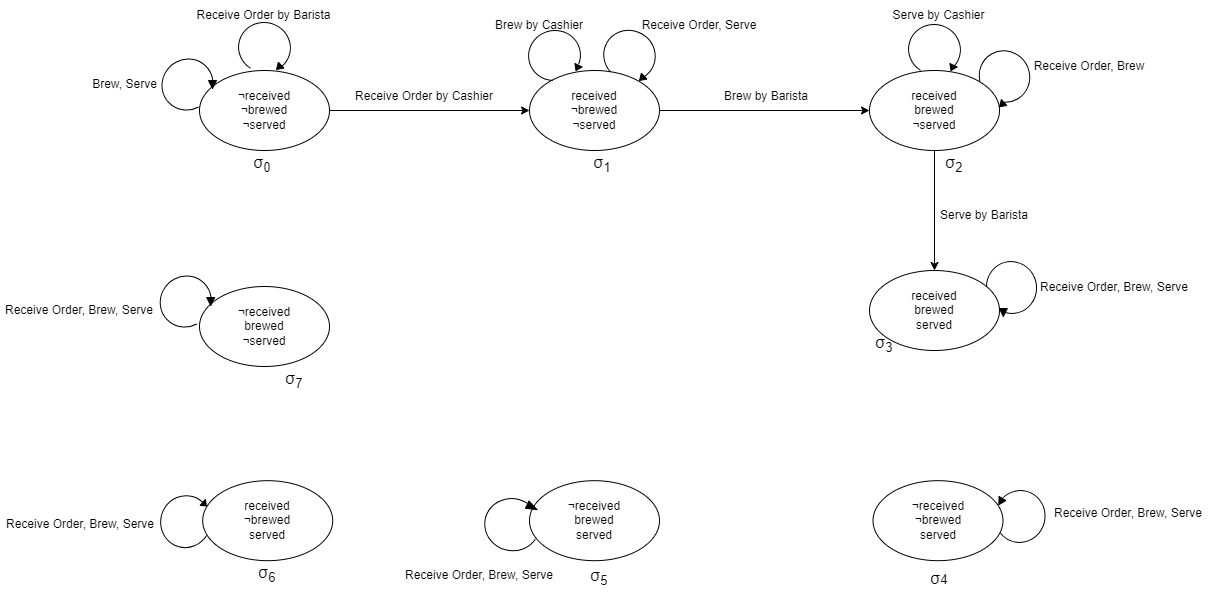
\includegraphics[width=1\linewidth]{coffeshop.png}
    \caption{Coffee orders - all possible transitions}
    \label{fig:coffee_order_transactions}
\end{figure}
Let us demonstrate an example of asking queries using the structure of the query language $\mathcal{QL_{CST}}$. 
Assume, that the initial state is $\sigma_0$ and the program $\mathcal{P}$ = ((\textit{Receive Order}, \textit{Cashier}),(\textit{Brew}, \textit{Barista}), (\textit{Serve}, \textit{Barista})).
Let us consider the following query statements:
\begin{enumerate}
  \item \textit{served} \textbf{after} ((\textit{Receive Order}, \textit{Cashier}),(\textit{Brew}, \textit{Barista}), (\textit{Serve}, \textit{Barista})).
  \item \textbf{Active} Cashier \textbf{in} ((\textit{Receive Order}, \textit{Cashier}),(\textit{Brew}, \textit{Barista}), (\textit{Serve}, \textit{Barista})).
\end{enumerate}
The program execution will consist of the following transitions: \\[0.5\baselineskip]
$\Psi((\text{Receive Order},Cashier),\sigma_0)$ = $\sigma_1$ \\[0.1\baselineskip]
$\Psi((\text{Brew}, Barista),\sigma_1)$ = $\sigma_2$ \\[0.1\baselineskip]
$\Psi((\text{Serve},Barista),\sigma_2)$ = $\sigma_3$ \\[0.7\baselineskip]
As it can be observed, after the program execution, the state $\sigma_3$ will hold. Due to that, query number one will retrieve a positive response (i.e. \textit{true}), 
as in the final state \textit{served} holds. 
On the other hand, the second query will respond with \textit{true} as  action performed by Agent \textit{Cashier} did changed the state of $\sigma_0$ into $\sigma_1$.
\section{Individual contribution}

\begin{enumerate}
    \item \textbf{Jianhao Luo} -- Theoretical part: 70\%  Example part: 30\%
    \item \textbf{Dmytro Narepekha} -- Theoretical part: 60\%  Example part:  40\%
    \item \textbf{Sabrila Trifebi Shina} -- Theoretical part: 50\%  Example part: 50\%
    \item \textbf{Suzzane Abiri} -- Theoretical part: 50\%  Example part: 50\%
\end{enumerate}
\end{document}
